\subsection{Interrelación Alumno - Alumno Curso Académico}

   \begin{description}
      \item[Definición] En esta interrelación se deja constancia de que un
      alumno puede estar matriculado durante un número indeterminado de cursos
      académicos.

      \item[Características] La interrelación presenta las siguientes
                             características:

         \begin{itemize}
            \item \textbf{Nombre:} A-AlCA
            \item \textbf{Tipo de la interrelación:} El tipo de entidad
                  Alumno Curso Académico es débil por identificación respecto al
                  tipo de entidad Alumno.
            \item \textbf{Cardinalidad de la interrelación:} 1:N
                  \begin{itemize}
                     \item Alumno: matriculado\_en (0,n)
                     \item Alumno Curso Académico: es\_un (1,1)
                  \end{itemize}
            \item \textbf{Número de atributos:} Ninguno.
         \end{itemize}

      \item[Diagrama] La figura \ref{diagramaA-AlCA} muestra el diagrama de la
                      interrelación.

      \item \begin{figure}[!ht]
            \begin{center}
            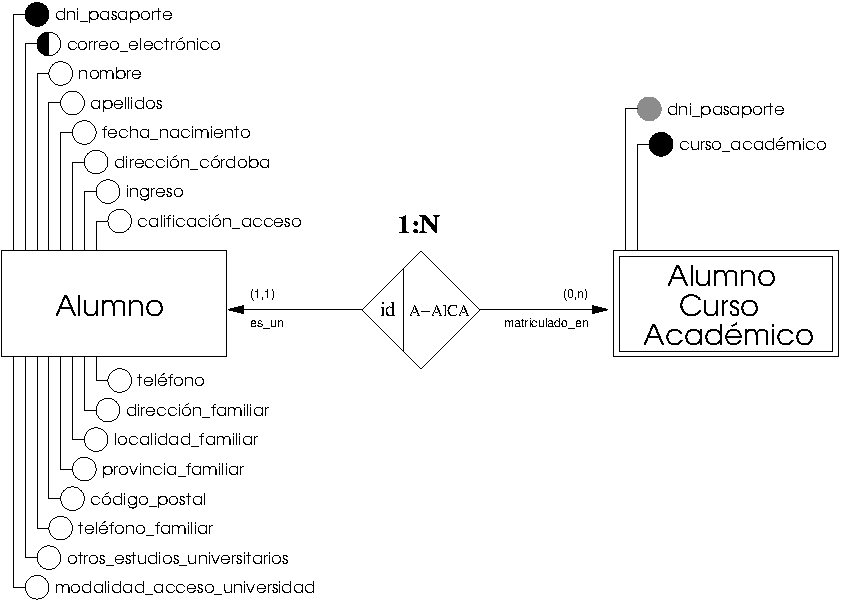
\includegraphics[]{07.Modelo_Entidad-Interrelacion/7.3.Analisis_Interrelaciones/diagramas/A-AlCA.pdf}
            \caption{Diagrama de la interrelación A-AlCA.}
            \label{diagramaA-AlCA}
            \end{center}
         \end{figure}

      \item[Ejemplo práctico del tipo de interrelación]

      \item \begin{center}
            \begin{tabular}{ | r r | }
            \hline
            \multicolumn{2}{ | c | }{\textbf{Tipo de interrelación A-AlCA}} \\
            \hline
            \textbf{Alumno} & \\
            dni\_pasaporte & 01234567A \\
            \hline
            \textbf{Alumno Curso Académico} & \\
            dni\_pasaporte & 01234567A \\
            id\_centro & 2008 \\
            \hline
            \end{tabular}
         \end{center}
   \end{description}
